% !TEX root = thesis.tex

%\section{Introduction}

\begin{abstract}

\end{abstract}
\tableofcontents
\listoffigures

\clearpage
\section{Introduction}
 At sufficiently high energies quarks and gluons are no longer bound to hadrons, but they form a deconfined state known as Quark-Gluon plasma (QGP). The main goal of heavy ion physics is the study of QGP and its properties.
One of the experimental observables that is sensitive to the properties of QGP is the azimuthal distribution of particles in the plane perpendicular to the beam direction. 

When nuclei collide at non-zero impact parameter (non-central collisions), their overlap region is asymmetric. This initial spatial asymmetry is converted via multiple collisions into an anisotropic momentum distribution of the produced particles. For low momentum particles ($\pt{} \lesssim 3$ \gevc), this anisotropy is understood to result from hydrodynamically driven flow of the QGP~\cite{Adcox:2004mh, Adams:2005dq, Ollitrault:1992, Heinz:2002, Shuryak:2009}. 

One way to characterize this anisotropy is with coefficients from a Fourier series parametrization of the azimuthal angle distribution of emitted hadrons. The second order coefficient, $v_2$ which is also known as elliptic flow, shows clear dependence on centrality. The collision geometry is mainly responsible for the elliptic flow. Higher harmonics don't depend that much on centrality. These higher harmonics carry information about the fluctuations in collisions. The event-by-event fluctuations have an increasing importance in measurements and it has been observed that measurements of elliptic flow in central collisions and measurements of higher order harmonics are consistent with the assumption that flow in these cases is mainly due to fluctuations~\cite{Jia:2012ve}.



At LHC energies  $\sqrt{s_{NN}}=2.76\mathrm{GeV}$ it has been observed that in general there is little difference to flow at RHIC energies. The $v_2$ coefficient is about 20\% greater at LHC than at RHIC, depending on the centrality bin. 
The particle identified $v_2$ for kaons and pions follows the same trend. However it was observed that for proton $v_2$ the quark number scaling does not work~\cite{Lacey:2012ma}. So far there is no agreement of why this scaling breaks down at LHC or why it works so well at RHIC energies.

\pagebreak
\subsection{Quantum chromodynamics}
\subsubsection{Foundation of QCD}
There are four known basic interactions in the universe: gravity, electromagnetic, weak and strong interactions. The standard model of particle physics includes three of these excluding the gravitational interaction. The theory of strong interactions is known as Quantum Chromodynamics (QCD).

The development of QCD began after the introduction of new powerful particle accelerators that were capable of particle physics research in the 1950s. Before this particles were mainly discovered from cosmic rays. Positrons, neutrons and muons were discovered in the 1930s and charged pions were discovered in 1947~\cite{}. The neutral pion was discovered in 1950~\cite{Bjorklund:1950}.

The Lawrence Berkeley National Laboratory started the Bevalac accelerator in 1954, Super Proton Synchrotron (SPS) in CERN began operating in 1959 and the Alternating Gradient Synchrotron at Brookhaven started in 1960. With an energy of $33\gev$ AGS was the most powerful accelerator of that time. By the beginning of 1960s several new particles had been discovered. These include antiprotons, antineutrons, $\Delta$-particles and the six hyperons ($\Xi^0$, $\Xi^-$, $\Sigma^{\pm}$, $\Sigma^0$ and $\Lambda$).

Facing this number of different particles started the search for symmetries. Already in 1932 Heisenberg~\cite{Heisenberg:1932} 
had proposed an isospin model to explain similarities between the proton and the neutron. In 1962 Gell-Mann and Ne'eman presented that particles sharing the same quantum numbers (spin, parity) could be organised using the symmetry of SU(3).~\cite{Gell-Mann:1962} Heisenberg's Isospin model followed the symmetry of SU(2). Using the SU(3) model known baryons and mesons could be presented as octets. This also lead to the discovery of the $\Omega^{-}$ particle since this was missing from the SU(3) decoupler that included heavier baryons. 

The most simple representation of SU(3) was a triplet. Inside this triplet particles would have electric charges $\nicefrac{2}{3}$ or $-\nicefrac{1}{3}$. These had not been however detected. In 1964 Gell-Mann~\cite{Gell-Mann:1964} and Zweig proposed that baryons and mesons would bound states of these three hypothetical triplet particles that Gell-Mann called quarks. Now we know that these are the $u$, $d$ and $s$ quarks. This original quark model was violating the Pauli exclusion principle. For example the $\Omega^{-}$ particle is comprised of three $s$ quarks which would have exactly the same quantum states. 

The first one to present the idea of colour was Greenberg already in 1964~\cite{Greenberg:1964}. In 1971 Gell-Mann and Frtizsch presented their model, which solved the antisymmetry problem. They added a colour quantum number to quarks, which separated quarks of the same species. In the new colour model the baryonic wave function became

\begin{equation}
\left( qqq\right)\rightarrow\left(q_rq_gq_b-q_gq_rq_b+q_bq_rq_g-q_rq_bq_g+q_gq_bq_r-q_bq_gq_r\right),
\end{equation}

The colour model was also supported by experimental evidence. The decay rate of a neutral pion with the addition of colours is

\begin{equation}
\Lambda\left(\pi^0\rightarrow\gamma \gamma\right) = \frac{\alpha^2}{2\pi}\frac{N_c^2}{3^2}\frac{m_\pi^3}{f_\pi^2}.
\end{equation} 

\noindent For $N_c=3$ this gives $7.75 \mathrm{eV}$ and the measured value is $(7.86\pm0.54)\,\mathrm{eV}$~\cite{Williams:1988sg}.

Another observable that combines the colour information also to the number of quark flavours is The Drell-Ratio $R$~\cite{Krolikowski:1974jx}

\begin{equation}
R=\frac{\sigma\left(e^++e^-\rightarrow\mathrm{hadrons}\right)}{\sigma\left(e^++e^-\rightarrow\mu^++\mu^-\right)}=N_c\sum_fQ_f^2.
\end{equation}

\noindent This ratio has the numerical value 2 when including the three light quarks $u$, $d$ and $s$. When the collision energy reaches the threshold of heavy quark ($c$ and $b$) production processes this increases to $\nicefrac{10}{3}$ (for $f=u,d,s,c$) and \nicefrac{11}{3} (for $f=u,d,s,c,b$). The threshold of $t\bar t$ production, $\sqrt{s}\approx350\gev$ has not been reached so far by any $e^+e^-$ colliders.

The colour model explained why no free quarks had been observed. Only colour neutral states are possible. The simplest ways of producing a colour neutral object are the combination of three quarks, and the combination of a quark-antiquark pair. These are known as baryons and mesons.

After the addition of colour the main ingredients of QCD had been established. The final quantum field theory of Quantum Chromodynamics formed quickly between 1972 and 1974. Main part of this was the work Gross, Wilczek, Politzer and George did for non-abelian gauge field theories~\cite{gross1973ultraviolet, politzer1973reliable, gross1973asymptotically, gross1974asymptotically, georgi1974electroproduction}. Gross, Wilczek and Politzer received the Nobel Prize in Physics for their work. The role of gluons was as a colour octet was presented by Fritzsch, Gell-Mann and Leutwyler in 1973~\cite{fritzsch1973advantages}. The theory had now 8 massless gluons to mediate the strong interaction.

However, these gluons had not been discovered. Indirect evidence of the existence had been seen 
 as it was observed that only about half of the momentum of protons was transported by the quarks~\cite{25gluons}. Direct evidence should be seen in electron-electron collisions as a third, gluonic, jet in addition to two quark jets. Three jet events were first seen in 1979 at the PETRA accelerator at DESY~\cite{Brandelik1979243, PhysRev.43.830, Berger1979418}.

\subsubsection{Asymptotic Freedom}
In Quantum Electrodynamics (QED) The electric charge is screened. In the vicinity of a charge, the vacuum becomes polarized. Virtual charged particle-antiparticle pairs around the charge are arranged so that opposing charges face each other. Since the pairs also include an equal amount opposite charge compared to the original charge the average charge seen by an observer at a distance is smaller. When the distance to the charge increases the effective charge decreases until the coupling constant of QED reaches the fine-structure constant $\alpha=\frac{1}{137}$. 

Contrary to QED QCD is a non-abelian theory. In other words the generators of the symmetry group of QCD, SU(3), do not commute. This has the practical consequence that gluons interact also with other gluons, whereas in QED the neutral carrier particles, photons, only interact with charged particles.
There is screening also in QCD because of the colour charges, but in addition to that there is antiscreening because of the gluon interactions. In QCD the antiscreening effect is stronger than screening. For larger distances to the colour charge the coupling constant is larger. This explains why no free colour charges can be observed. When the distance between charges increases the interaction strengthens until it is strong enough to produce a new quark-antiquark pair. 

On the other hand, at very small distances the coupling constant approaches 0. This is called asymptotic freedom. For large energies and small distances the coupling constant is negligible. In 1975 Collins\cite{Collins:1975} predicted a state where individual quarks and gluons are no longer confined into bound hadronic states. Instead they form a bulk QCD matter that Edward Shuryak called Quark-Gluon plasma in his 1980 review of QCD and the theory of superdense matter~\cite{Shuryak:1980}. QGP can be seen as a separate state of matter. A schematic view of a phase diagram for QCD matter is shown in Fig. \ref{fig:QCDphase}. 

\begin{figure}[htbp]
\centering
%\includegraphics[width=0.9\textwidth]{pics/qcd_ms_high}
\includegraphics[width=0.5\textwidth]{pics/QCDphase2}
\caption[QCD phase diagram]{A schematic outline for the phase diagram of QCD matter at ultra-high density and temperature. The quark chemical potential $\mu$ that is on the x-axis represents the imbalance between quarks and antiquarks. At zero temperature this corresponds to the number of quarks but at higher temperatures there are also additional pairs of quarks and antiquarks. Along the horizontal axis the temperature is zero, and the density is zero up to the onset transition where it jumps to nuclear density, and then rises with increasing $\mu$.  Neutron stars are in this region of the phase diagram, although it is not known whether their cores are dense enough to reach the quark matter phase. Along the vertical axis the temperature rises, taking us through the crossover from a hadronic gas to the quark-gluon plasma. This is the regime explored by high-energy heavy-ion colliders.~\cite{Rajagopal:2001}}
\label{fig:QCDphase}
\end{figure}


In the early universe at the age of $10^{-6}\mathrm{s}$ after the Big Bang the conditions preferred the existence of QGP instead of hadronic matter. Nowadays bulk QCD matter, its properties and its phase transitions between hadronic matter and the quark-gluon plasma (QGP) can be explored in the laboratory, through collisions of heavy atomic nuclei at ultra-relativistic energies. The study of QCD matter at high temperature is of fundamental and broad interest. The phase transition in QCD is the only phase transition in a quantum field theory that can be probed by any present or foreseeable technology. 

One important property of the QGP is the shear viscosity to entropy ratio, $\nicefrac{\eta}{s}$. It is believed that this ratio has an universal minimum value of $\nicefrac{1}{4\pi}\approx 0.8$, which holds for all substances. This limit would be reached in the strong coupling limit of certain gauge theories~\cite{Kovtun:2004de}. The temperature dependance of the ratio is shown in Fig. \ref{fig:etas}. The minimum value of $\nicefrac{\eta}{s}$ is found in the vicinity of the critical temperature, $T_c$~\cite{PhysRevLett.98.092301}. Finding the $\nicefrac{\eta}{s}$ values in QGP matter would therefore also provide a way of determining the critical point of QCD matter.

The $\nicefrac{\eta}{s}$ value for the matter created in Au-Au collisions at RHIC ($\sqrt{s_{NN}}$)  has been estimated to be $0.09\pm0.015$~\cite{PhysRevLett.98.092301}, which is very close to the lowest value for a wide class of thermal quantum field theories~\cite{Kovtun:2004de} for all relativistic quantum field theories at finite temperature and zero chemical potential. This suggests that the the matter created goes through a phase where it is close to the critical point of QCD.

\begin{figure}[htb]
\centering
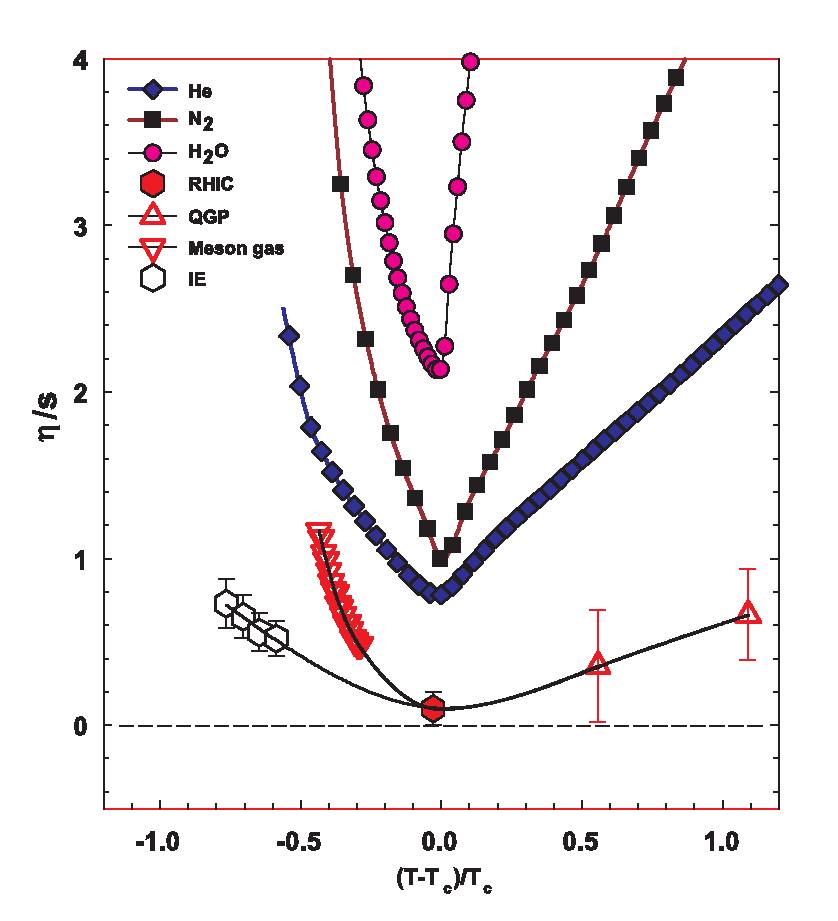
\includegraphics[width=0.5\textwidth]{pics/eta-s-vs-t-tc3}
\caption[$\eta/s$ vs $(T-T_c)/T_c$]{\label{fig3}$\eta/s$ as a function of $(T-T_c)/T_c$ for several substances as indicated.
	The calculated values for the meson-gas have an associated error 
	of $\sim$ 50\% %~\cite{Chen:2006ig}. 
	The lattice QCD value $T_c = 170$~MeV %~\cite{Karsch:2000kv} 
	is assumed for nuclear matter. The lines are drawn to guide the eye.~\cite{PhysRevLett.98.092301}
}
\label{fig:etas}

\end{figure}

\FloatBarrier
\pagebreak
\subsection{Heavy ion physics}
The Quark Gluon Plasma (QGP) is experimentally accessible by colliding heavy ions at high energies. Nowadays research of Heavy-Collisions is mainly performed at two particle colliders; the The Relativistic Heavy Ion Collider (RHIC) at BNL in New York, USA and he Large Hadron Collider (LHC) at CERN in Switzerland. Energy densities at these colliders should be enough to produce QGP and convincing evidence of the creation has been seen at both colliders.

The development of heavy ion physics is strongly connected to the development of particle colliders. Experimental study of relativistic heavy ion collisions has been carried out for three decades, beginning with the Bevalac at Lawrence Berkeley National Laboratory (LBNL)~\cite{Lofgren_1975}, and continuing with the AGS at Brookhaven National Laboratory (BNL)~\cite{Barton:1987}, CERN SPS~\cite{Vitev:2002pf}, RHIC at BNL and LHC at CERN. The first colliders could not produce enough energy to create QGP matter so they could only probe the hadronic state. 

The collective motion of matter in a heavy-ion collision has been modeled using several models e.g. the Blast wave Model~\cite{PhysRevC.84.064905} has been used succesfully. Another model growing in popularity is the hydrodynamical approach which is further discussed in section \ref{sec:hydro}.

\subsubsection{History}
The first heavy-ion collisions were done at the Bevalac experiment at the Lawrence Berkeley National Laboratory~\cite{Lofgren_1975} and at the Joint Institute for Nuclear Research in Dubna~\cite{kovalenko1994status} at energies up to 1$\gev$ per nucleon.
In 1986 the Super Proton Synchrotron (SPS) at CERN started to look for QGP signatures in O+Pb collisions. The center-of-mass energy per colliding nucleon pair $\left(\sqrt{s_{NN}}\right)$ was 19.4 GeV~\cite{Vitev:2002pf}. These experiments did not find any decisive evidence of the existence of QGP. In 1994 a heavier lead (Pb) beam was introduced for new experiments at $\sqrt{s_{NN}}\approx 17\; \mathrm{GeV}$. At the same time the Alternating Gradient Synchrotron (AGS) at BNL, Brookhaven collided ions up to $\mathrm{^{32}S}$ with a fixed target at energies up to $28\gev$~\cite{Barton:1987}. Although the discovery of a new state of matter was reported at CERN, these experiments provided no conclusive evidence of QGP. Now SPS is used with 400 GeV proton beams for fixed-target experiments, such as the SPS Heavy Ion and Neutrino Experiment (SHINE)~\cite{Grebieszkow:2013nza}, which tries to search for the critical point of strongly interacting matter.

The Relativistic Heavy Ion Collider (RHIC) at BNL in New York, USA started its  operation in 2000. The top center-of-mass energy per nucleon pair at RHIC, 200 GeV, was reached in the following years. The results from the experiments at RHIC have provided a lot of convincing evidences that QGP was created~\cite{Adcox:2004mh, Adams:2005dq, Arsene:2004fa, Back:2004je}. The newest addition to the group of accelerators capable of heavy-ion physics is the Large Hadron Collider (LHC) at CERN, Switzerland. LHC started operating in November 2009 with proton-proton collisions. First Pb-Pb heavy ion runs started in November 2010 with $\sqrt{s_{NN}}=2.76\; \mathrm{TeV}$,  over ten times higher than at RHIC. Among the six experiments at LHC, the Large Ion Collider Experiment (ALICE) is dedicated to heavy ion physics. Also CMS and ATLAS have active heavy ion programs. 




